\subsection{Layers}
\label{sec:layers}

\paragraph{Layer size}

\begin{figure}[!t]
	\subfigure[CDF of layer size]{\label{fig_layer_size}
		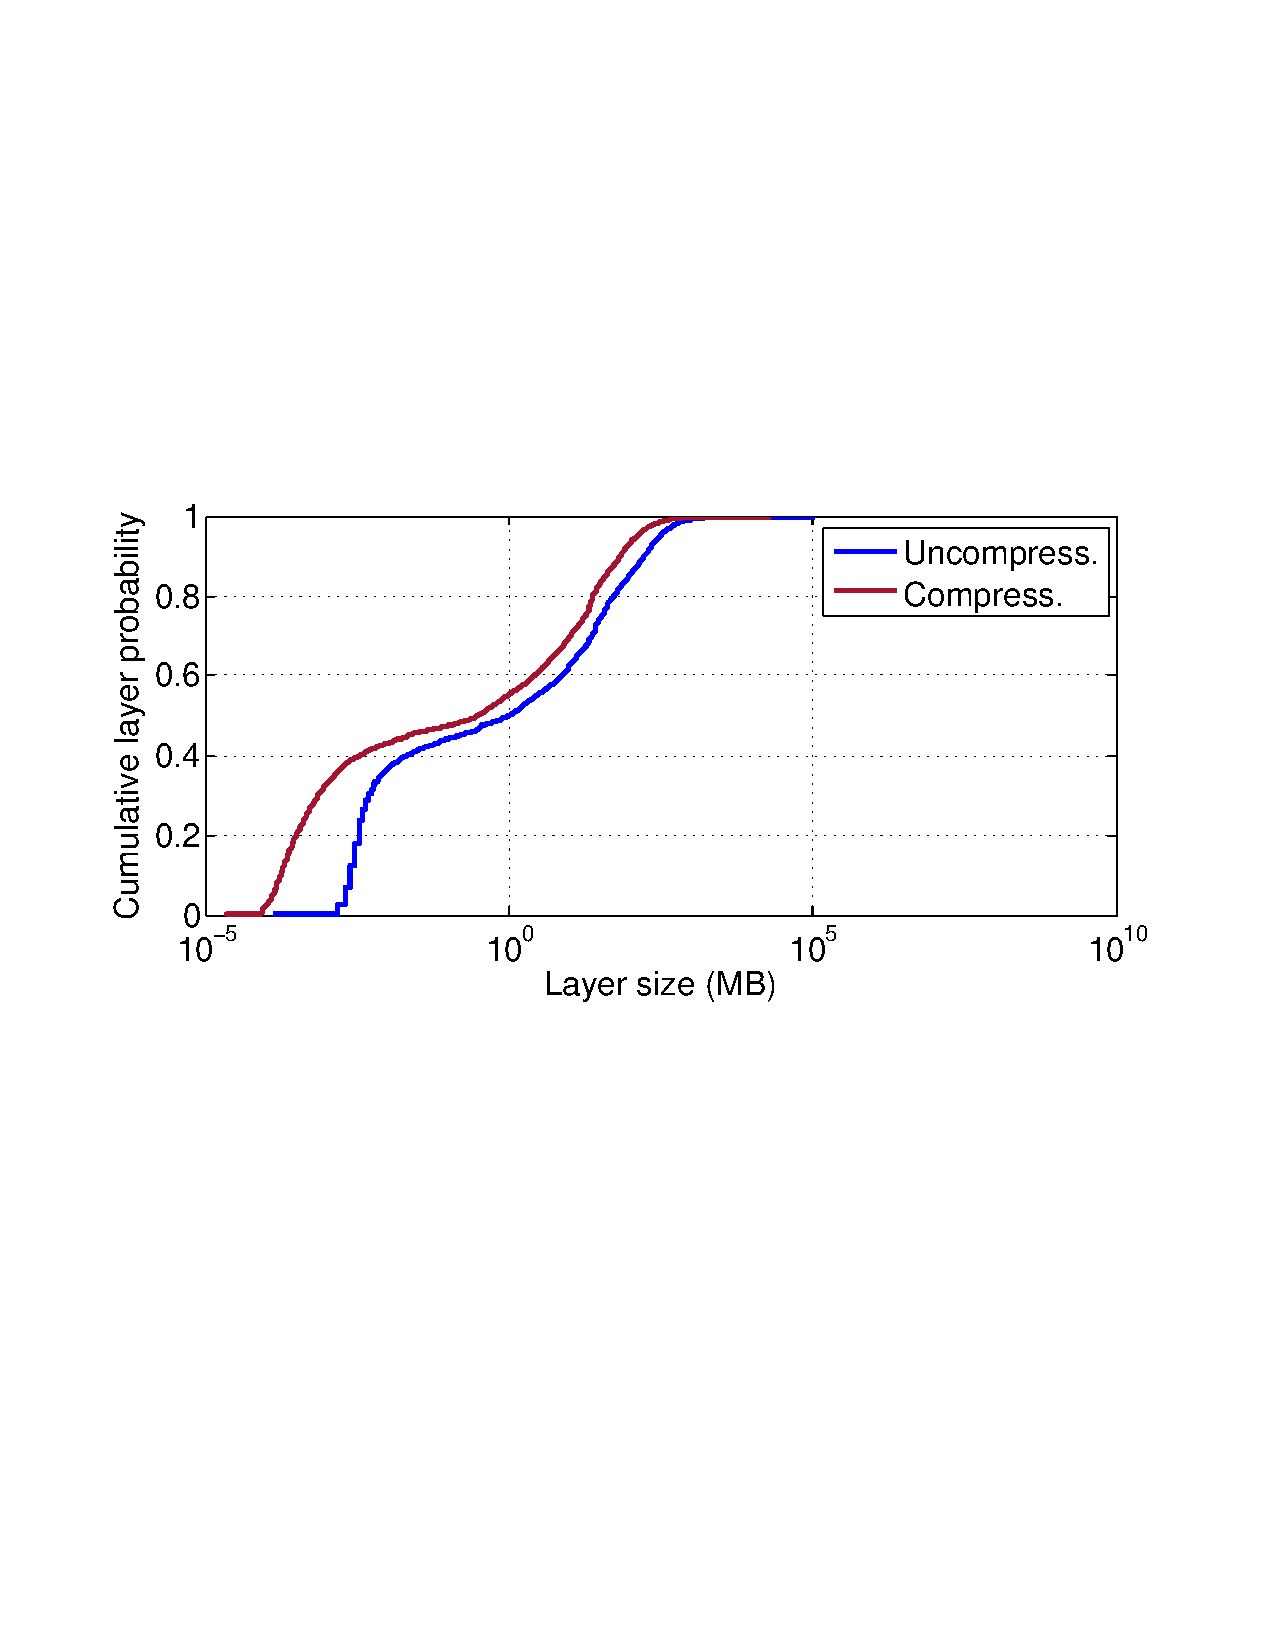
\includegraphics[width=0.4\textwidth]{graphs/layer-size-cdf.pdf}
		}
		\centering
		\subfigure[CDF of image size]{\label{fig_image_size}
			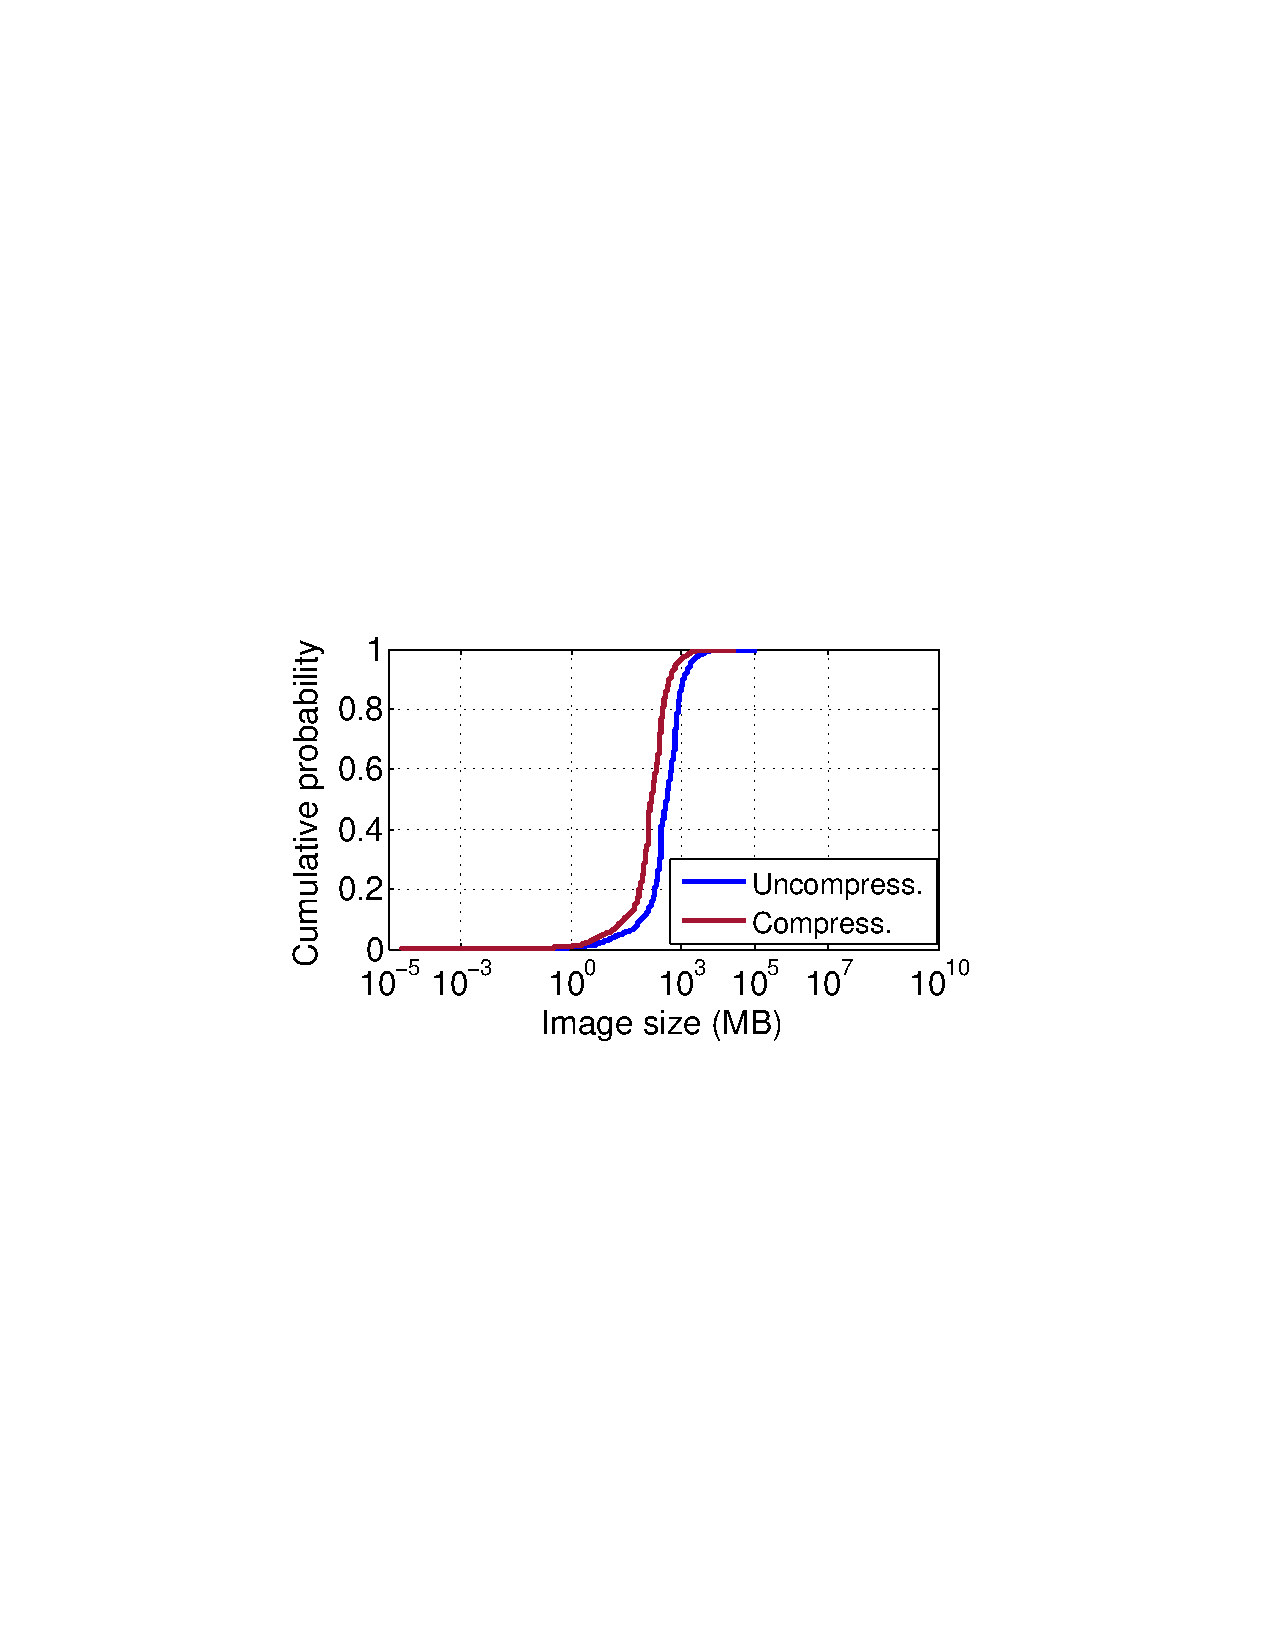
\includegraphics[width=0.4\textwidth]{graphs/image-size-cdf.pdf}%
			}
			
			\caption{Image/layer size distribution}
			\label{fig:image-layer-size}
			\end{figure}

\paragraph{Layer directory depth}
%\nancomment{fs metadata overhead}

\begin{figure}[!t]
	\centering
	\subfigure[CDF of layer depth]{\label{fig_reference_cnt_cdf}
		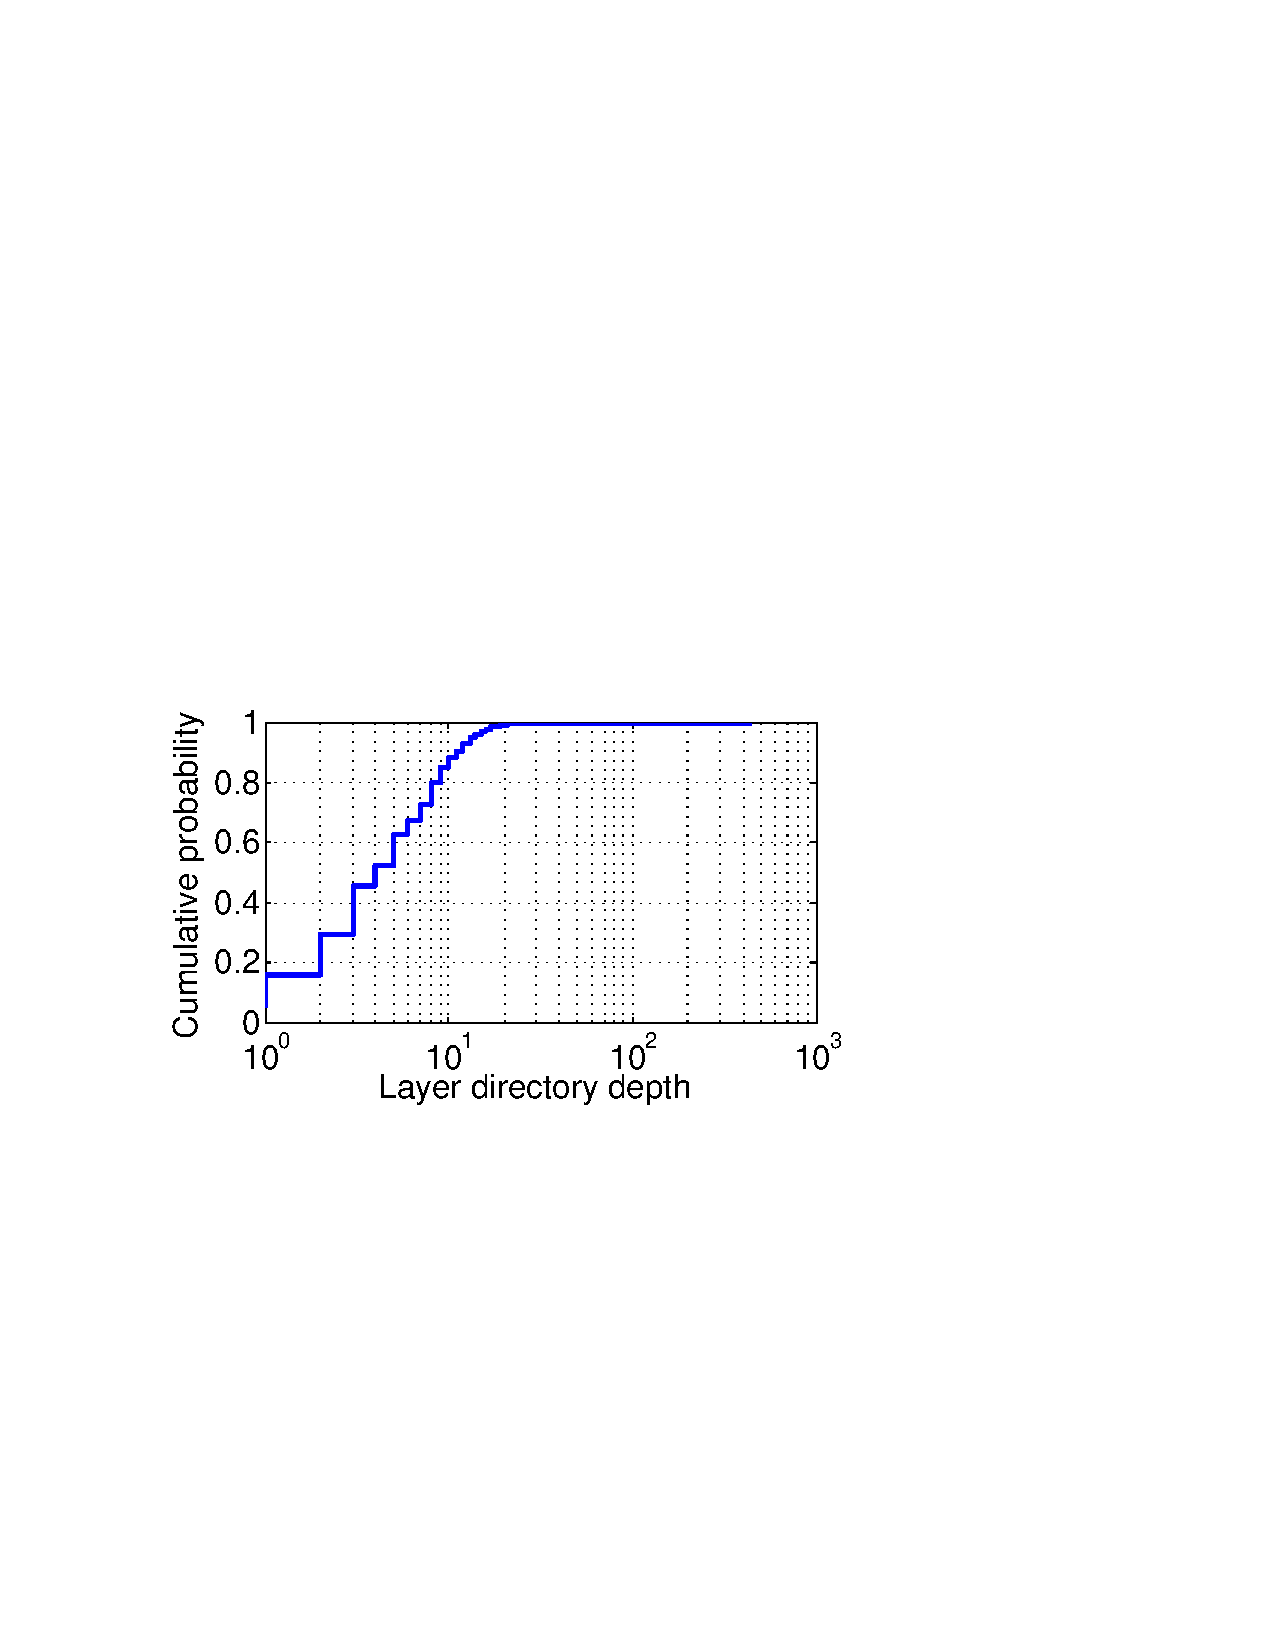
\includegraphics[width=0.21\textwidth]{graphs/layer-depth-cdf.pdf}%
	}
	\subfigure[Histogram of layer depth]{\label{fig_reference_cnt_pdf}
		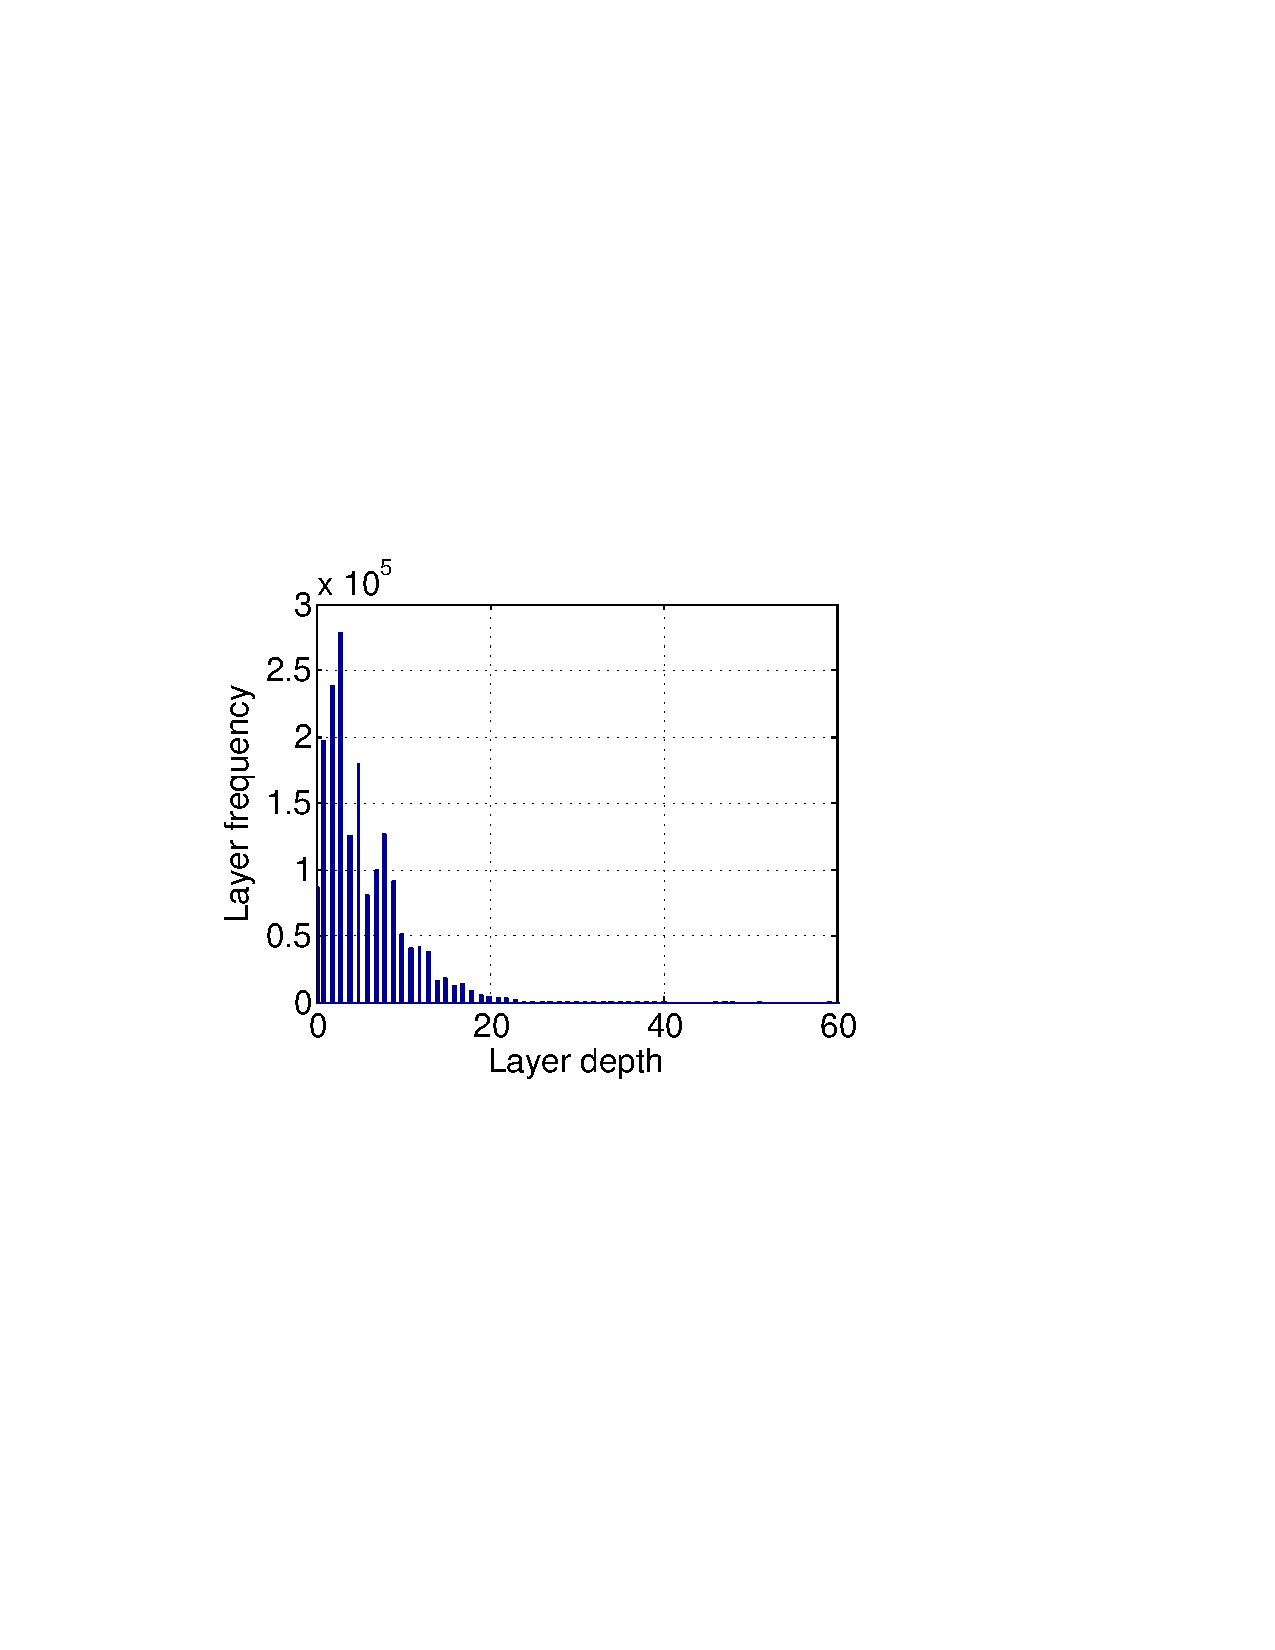
\includegraphics[width=0.21\textwidth]{graphs/layer-depth-pdf.pdf}
	}
	\caption{Layer depth distribution}
	\label{fig:reference-cnt}
\end{figure}

\paragraph{Directory count and File count}
%\nancomment{how union fs handle so large dirs}
\begin{figure}
	\centering
	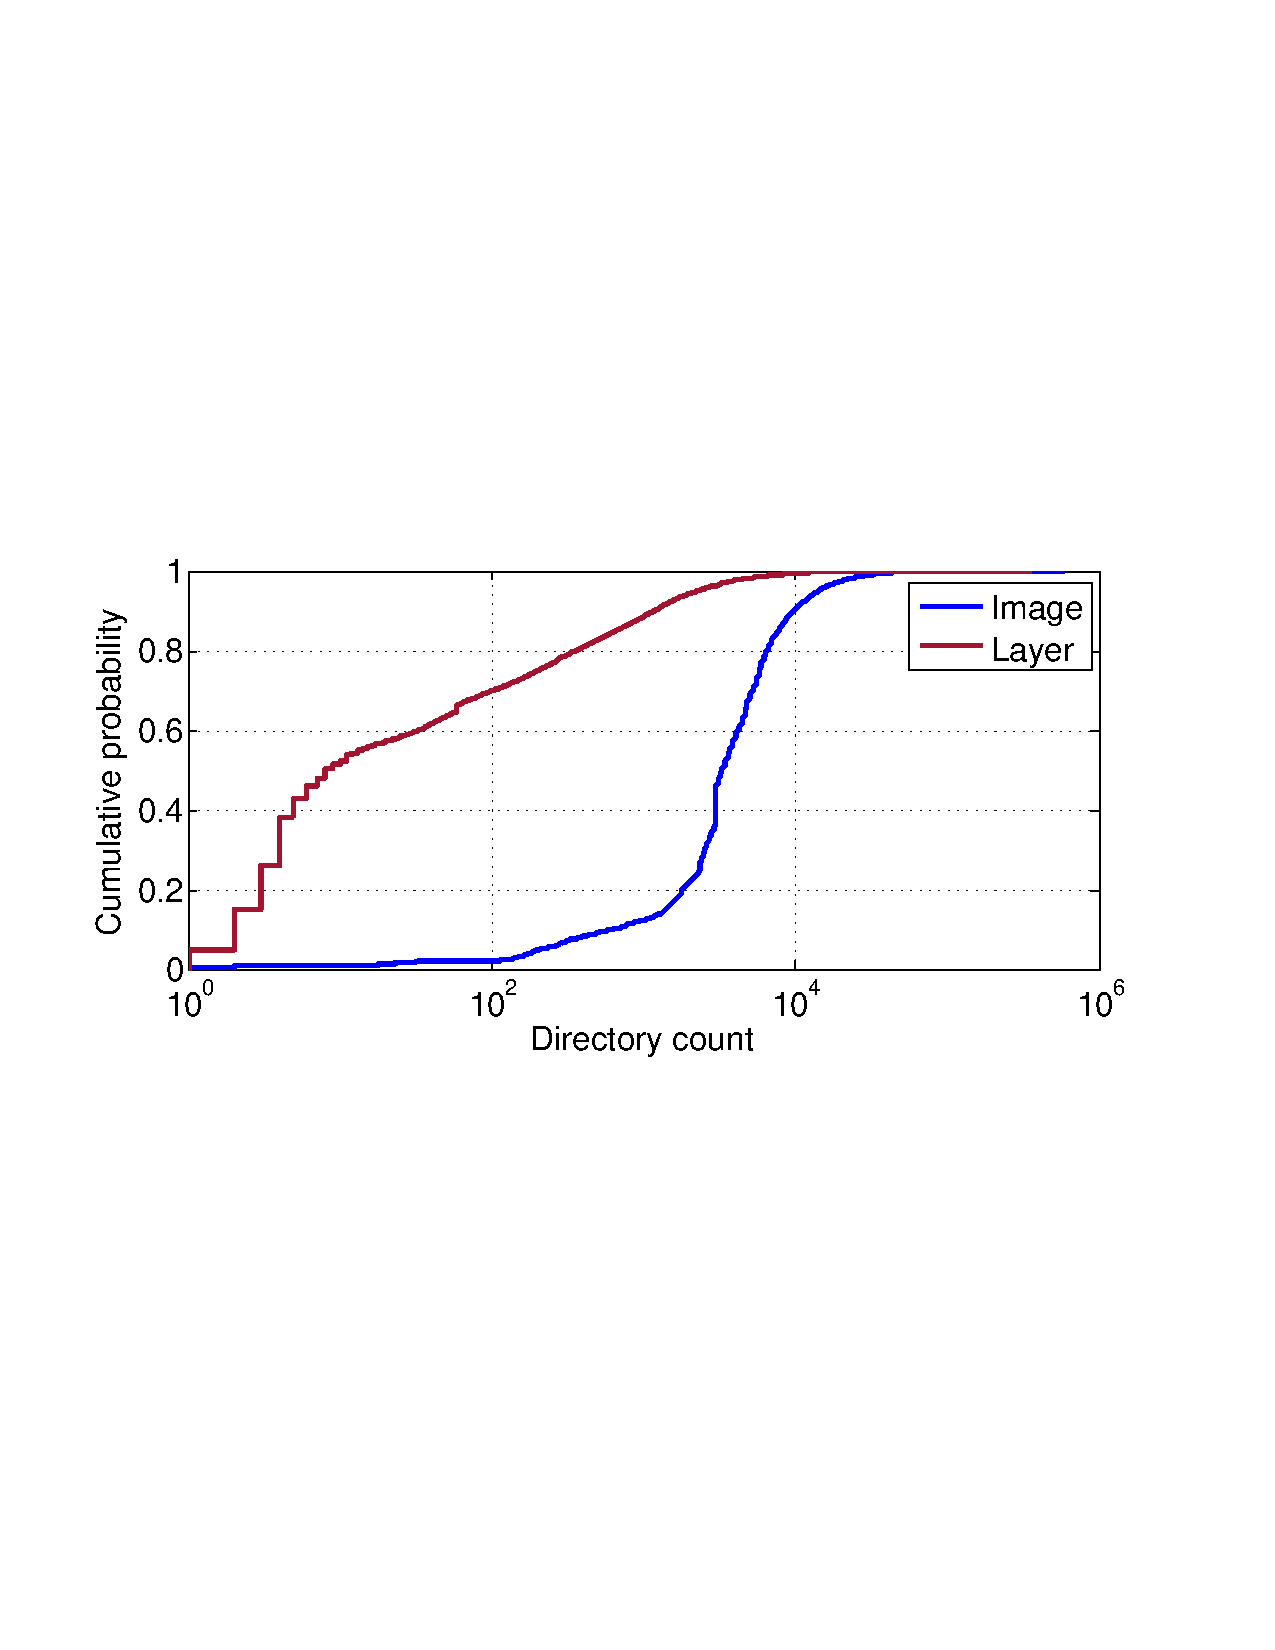
\includegraphics[width=0.4\textwidth]{graphs/dir-cnt-cdf.pdf}
	\caption{CDF of directory count per image/layer.
	}
	\label{fig:reference-cnt}
\end{figure}

\begin{figure}[!t]
	\centering
	\subfigure[Histogram of directory count per image]{\label{fig_reference_cnt_cdf}
		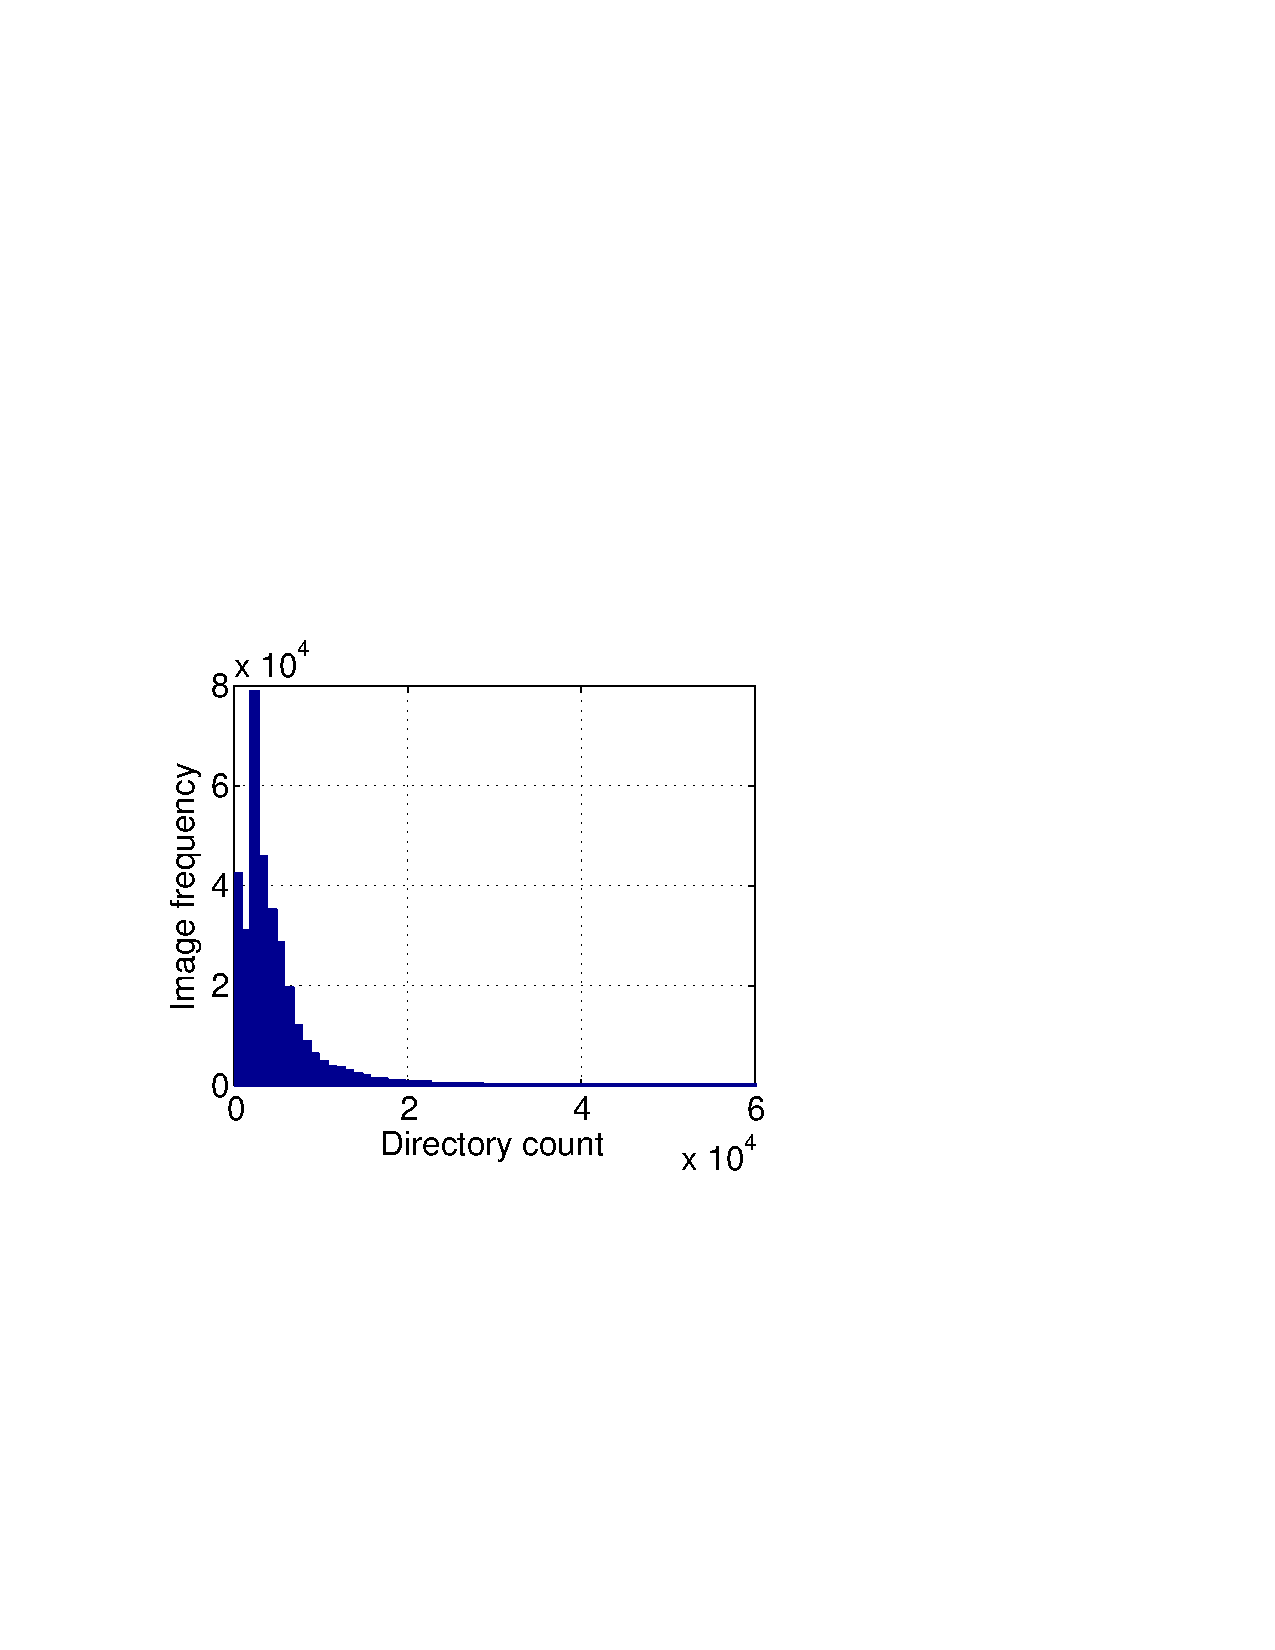
\includegraphics[width=0.2\textwidth]{graphs/image-dir-cnt-pdf.pdf}%
	}
	\subfigure[Histogram of directory count per layer]{\label{fig_reference_cnt_pdf}
		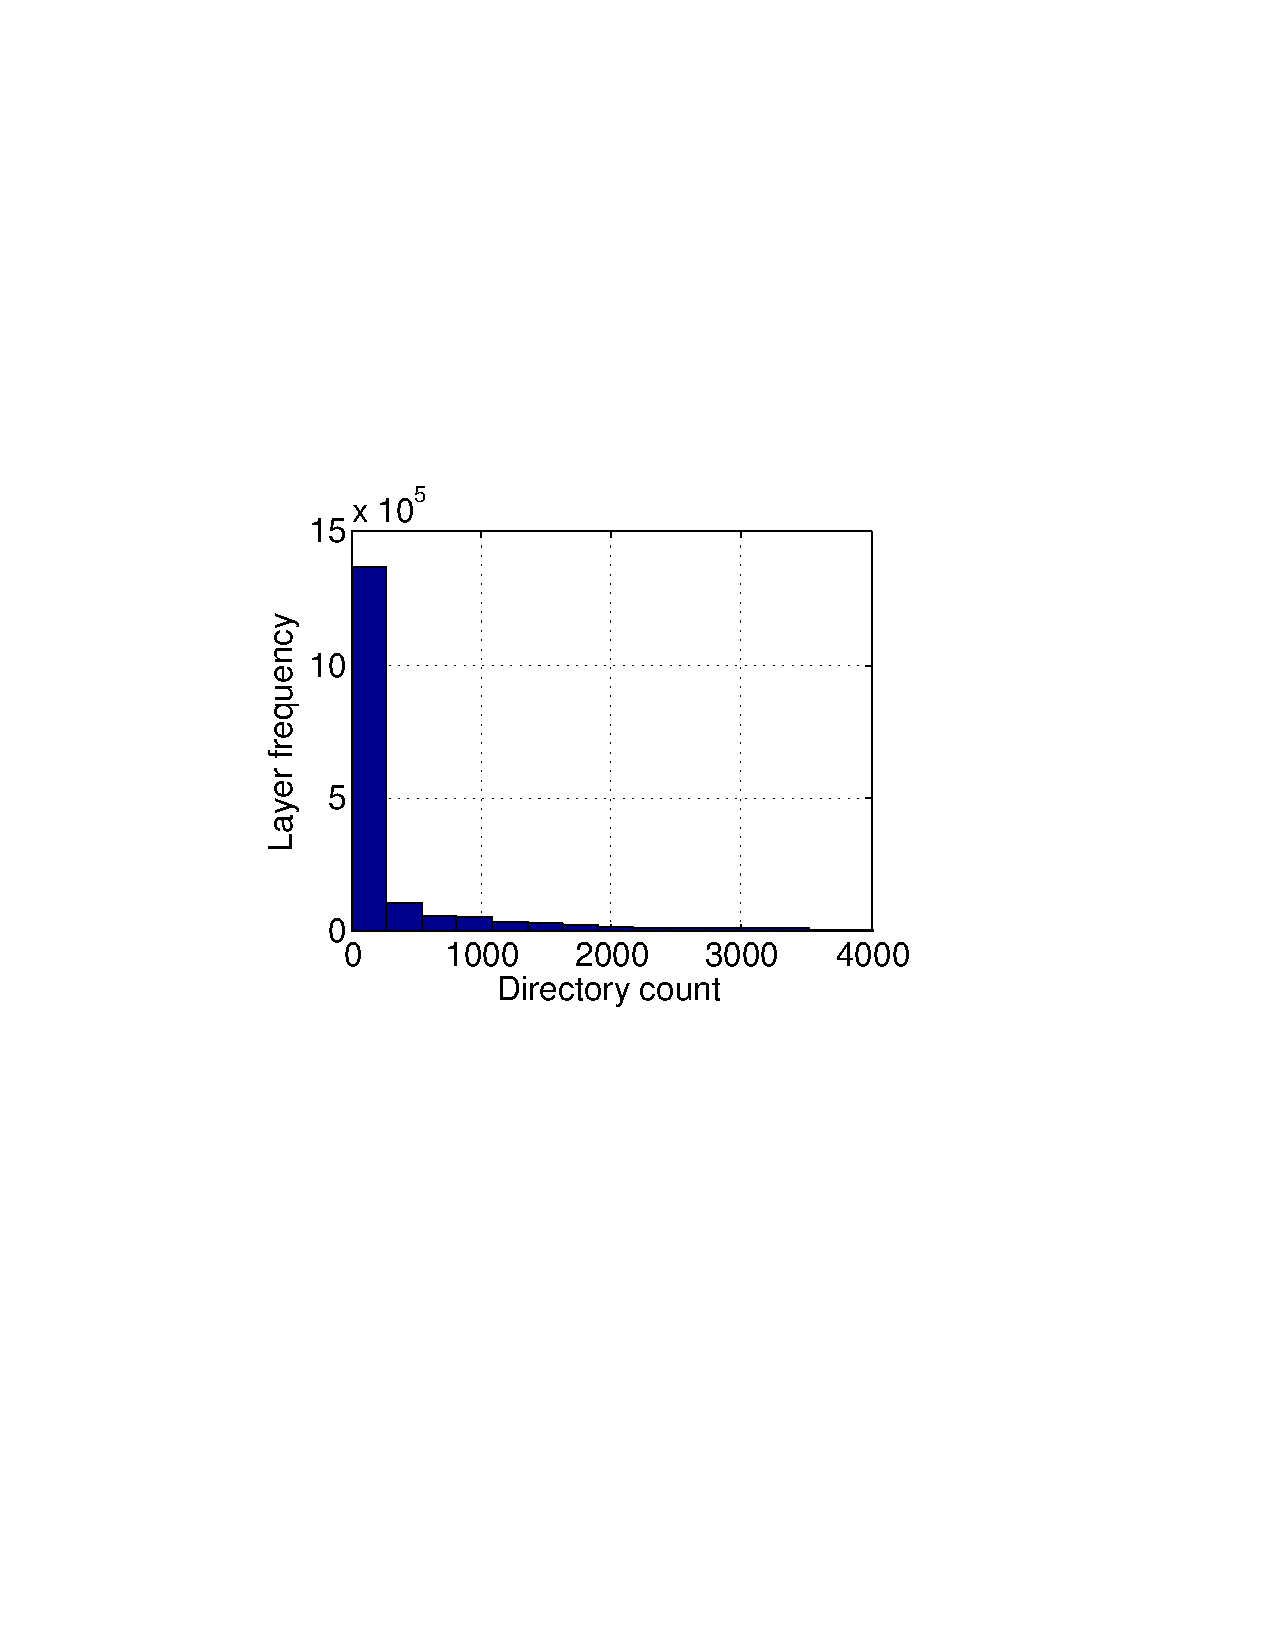
\includegraphics[width=0.22\textwidth]{graphs/layer-dir-cnt.pdf}
	}
	\caption{Histogram of directory count distribution}
	\label{fig:reference-cnt}
\end{figure}

Next, we look at the directory (Figure~\ref{fig-dir}) and file count
(Figure~\ref{fig-file}) in images to determine if deploying images requires
handling of large amounts of metadata. Looking at directories, we see that 90\%
of images have less than 7,344 directories while the median is at 296. For
files, 90\% of images have less than 64,780 files with a median of 1,090.

This is consistent with our analysis of layer-based file and directory counts
and the number of layers per image. Again, we conclude that most images do not
require an extensive amount of metadata when being deployed as file and
directory counts are low except for few outliers.

\paragraph{File count} 
%\nancomment{still metadata overhead}
\begin{figure}
	\centering
	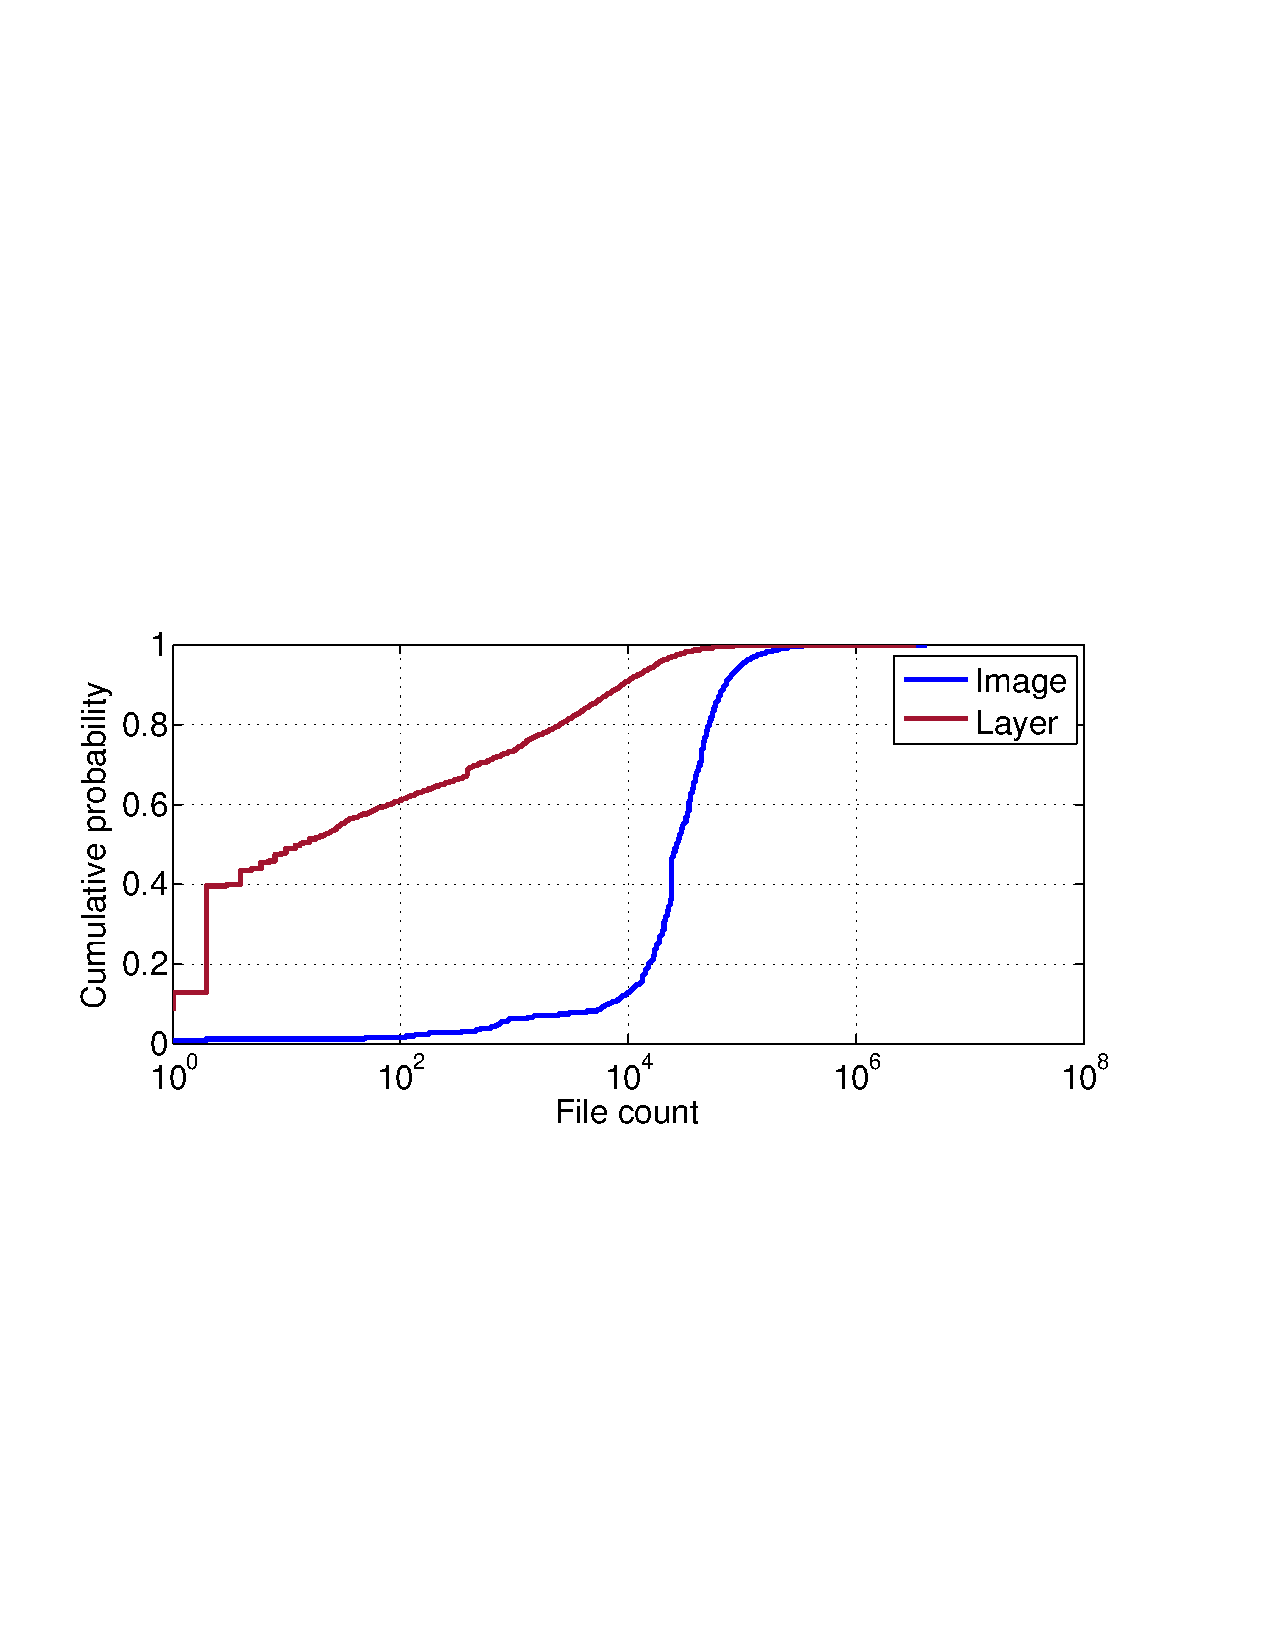
\includegraphics[width=0.4\textwidth]{graphs/file-cnt-cdf.pdf}
	\caption{CDF of file count per image/layer.
	}
	\label{fig:reference-cnt}
\end{figure}

\begin{figure}[!t]
	\centering
	\subfigure[Histogram of directory count per image]{\label{fig_reference_cnt_cdf}
		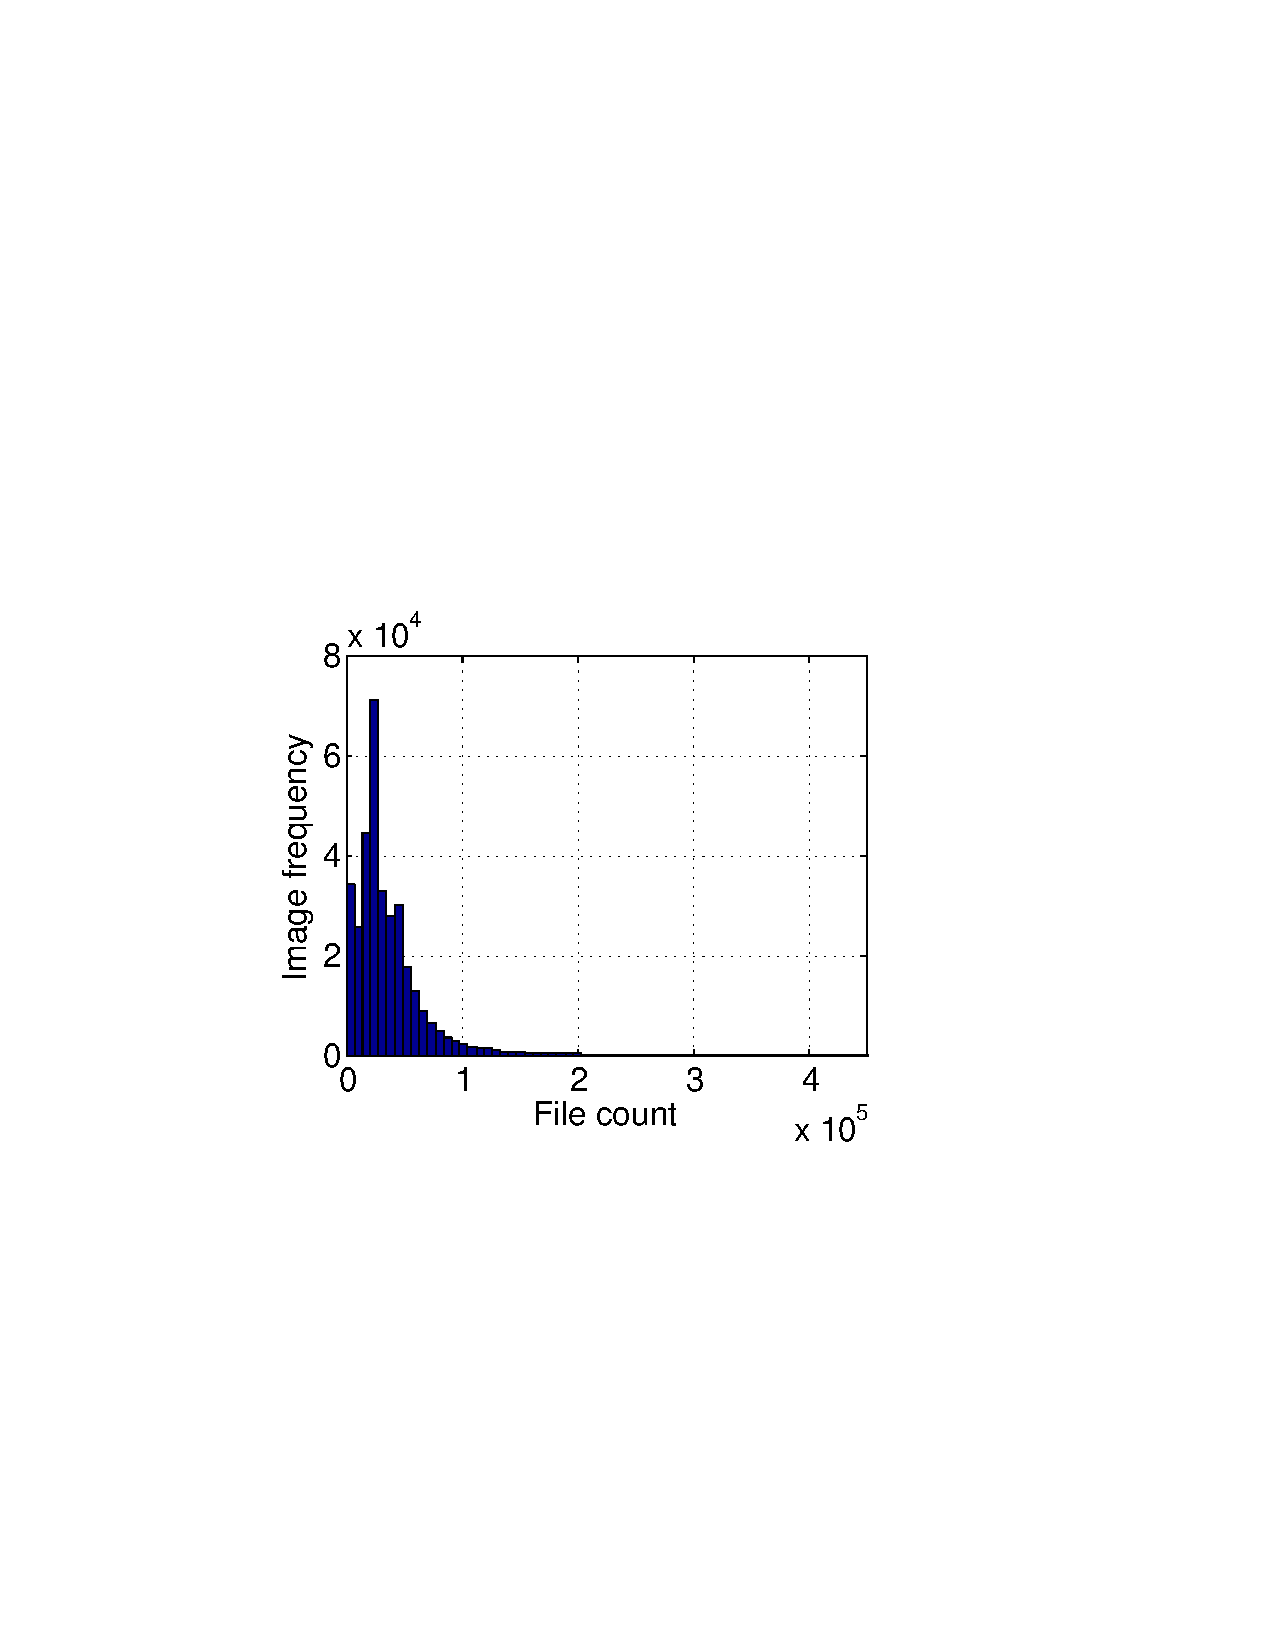
\includegraphics[width=0.21\textwidth]{graphs/image-file-cnt-pdf.pdf}%
	}
	\subfigure[Histogram of directory count per layer]{\label{fig_reference_cnt_pdf}
		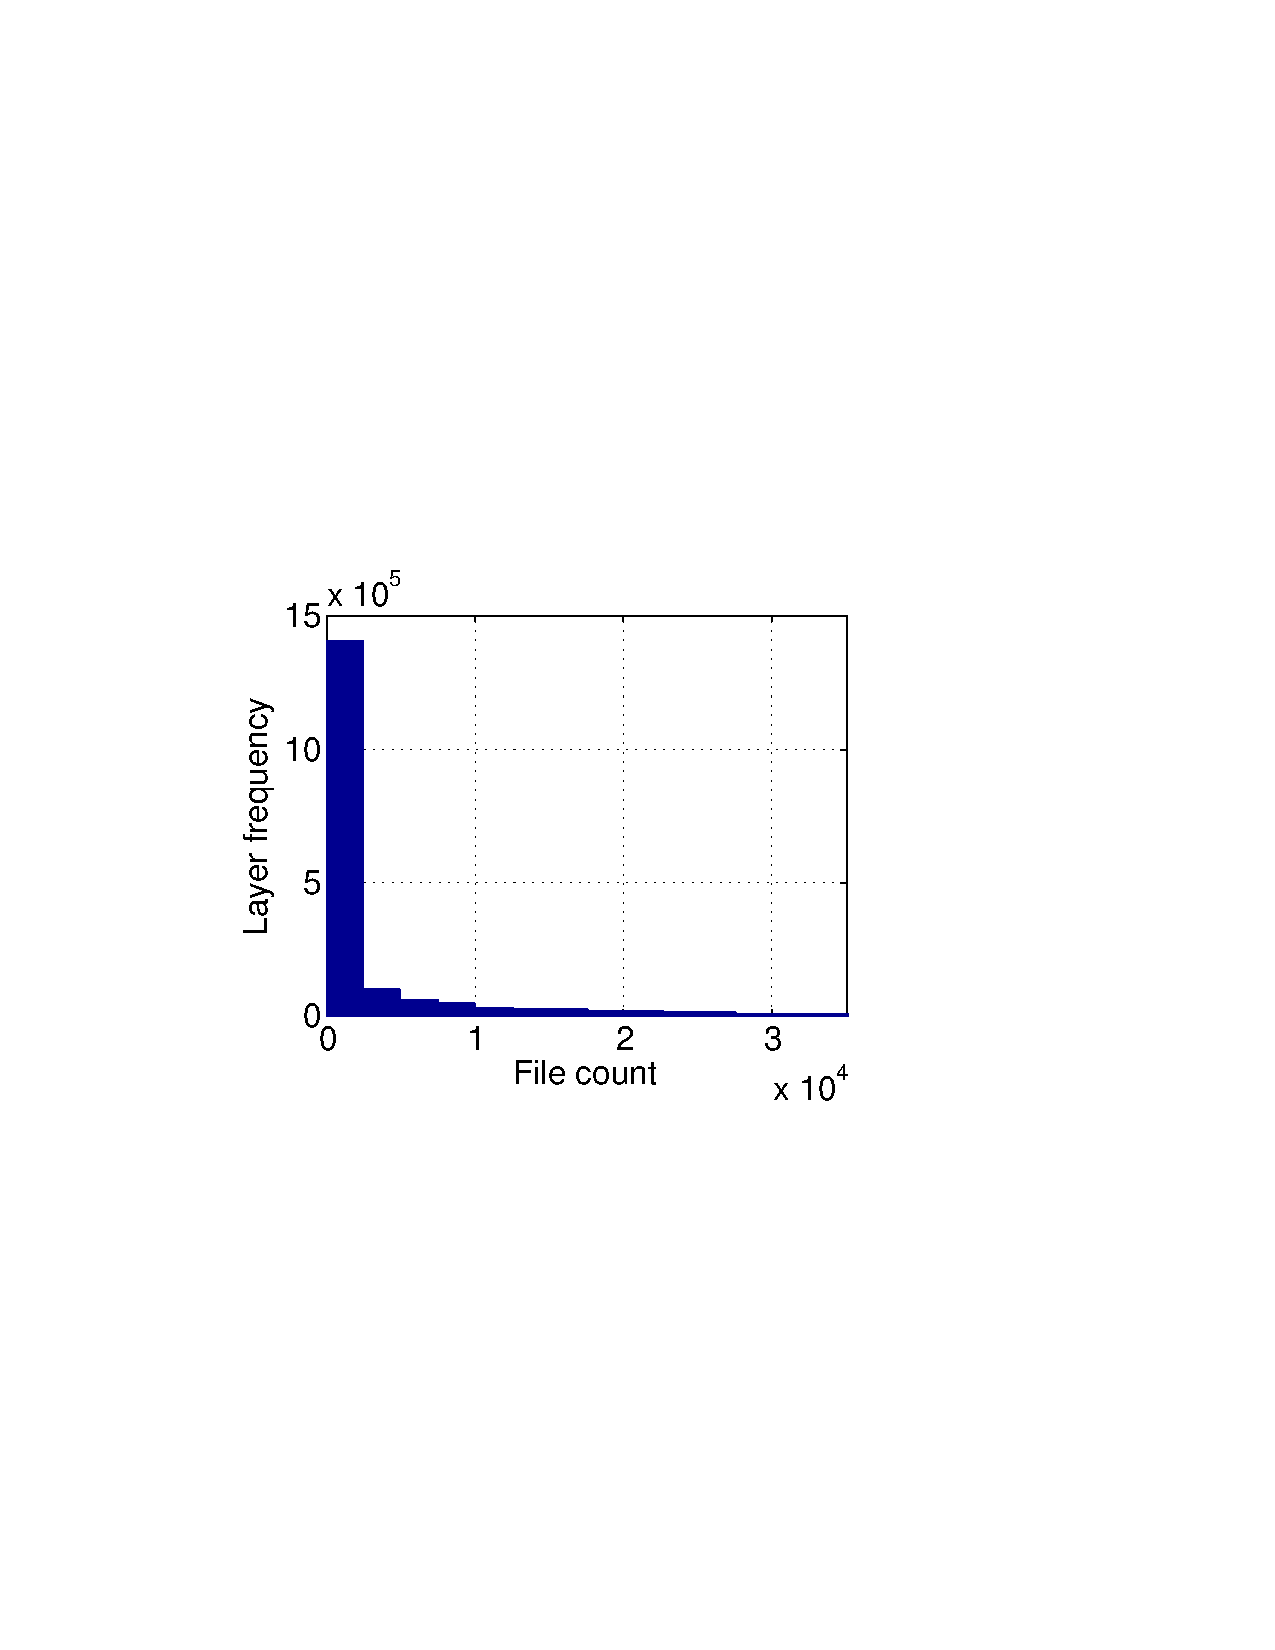
\includegraphics[width=0.22\textwidth]{graphs/layer-file-cnt-pdf.pdf}
	}
	\caption{Histogram of directory count distribution}
	\label{fig:reference-cnt}
\end{figure}

Lastly, we look at file and directory metrics in layers.
Figure~\ref{fig_file_cnt} and~\ref{fig_dir_cnt} show the CDFs of file and
directory counts in all layers, respectively.
%
The results show that 90\% of layers contain less than 7,410 files while half
of the layers have less than 30 files.
%
We also found that 27\% of the layers only have a single file while 7\% even
showed no files at all. We currently do not know the exact reason for the
layers without files, but one theory is that these layers use Docker volumes to
store all requred files (including executables).
% plan to investigate their corresponding images in the future.
%\nancomment{The layers are not empty since it could have directories}.
On the other hand, the largest layer contains 826,196 files and was part of a
Debian image.
%
%The average is 2,200.
%
For directories, 90\% of the layers have less than 826 directories and half of
the layers consist of less than 11 directories. We again observe a wide range
with a minimum of a single directory and a maximum of 111,940. The layer with
the most directories was part of the \textit{conjurinc/developer-quiz} image.

%\paragraph{Directory depths}

%After extracting and unpacking gzip compressed layer archival files,
Besides the count, we also calculate the maximum directory depth for each layer
(Figure~\ref{fig_layer_depth}).
%
Around 90\% of all layers have a directory depth less than 10 while for 50\% of
the layers, the directory depth is less than 4. 
%
The most frequent directory depth is 3 with 313,000 layers showing this depth
value (Figure~\ref{fig_hist_layer_depth}).
%
%About 313,000 layers' layer directory depth is 3, which is the peak value in
%the figure.
%
%The maximum repeat count is 444 while the median is 4. The average is ~5.

This analysis shows that the majority of layers consists only of a small number
of files and does not contain deeply nested directory hierarchies. Hence,
except a few outliers, unpacked layers do not require a large amount of
metadata from the storage system.